\documentclass[a4paper]{report}

%%%% Manual variants (JA or AJS)
\usepackage{etoolbox}
\newbool{AJS}
% Change this for different manual versions.
\setbool{AJS}{true}
% Shortcut commands
\newcommand{\AJSonly}[1]{\ifbool{AJS}{#1}{}}
\newcommand{\JAonly}[1]{\ifbool{AJS}{}{#1}}
\newcommand{\variant}{\ifbool{AJS}{AJS 37}{JA 37D}}

\newcommand{\versionnumber}{4.319}


% Todos:
% features.txt in the root directory

\usepackage[english]{babel}
\usepackage[utf8]{inputenc}
\usepackage[T1]{fontenc}
\usepackage{menukeys}
\usepackage{graphicx}
\usepackage{hyperref}
\usepackage{wallpaper}
\usepackage{xcolor}
\usepackage{geometry}
\usepackage{pdflscape}
\usepackage{gensymb}
\usepackage{multicol}
\usepackage{enumitem}
\usepackage{cleveref}
\usepackage{alltt}

\pagestyle{headings}

\usepackage{titlesec}
\titleformat{\chapter}[hang]{\bfseries\Huge}{\thechapter{}.}{1.2ex}{}
\titlespacing{\chapter}{0pt}{*0}{*3}

\setcounter{tocdepth}{1}


\begin{document}
\newgeometry{bottom=2cm}
\ThisCenterWallPaper{1.0}{images/title}
\begin{titlepage}
  \centering
  \sf
  {\Huge Saab \variant{} Viggen}
  \\[1cm]
  {\Huge FlightGear Flight Manual}
  \\[16cm]
  \color{white}
  \emph{Model by}\\
  Anders Lejczak, Justin Nicholson, Enrico Castaldi,\\
  Joshua Davidson, Nicola B.\ Bernardelli, Isaac Protiva,\\
  Colin Geniet, Nikolai V.\ Chr.\\[0.2cm]
  \emph{Manual by}\\
  Colin Geniet, Rick Gruber-Riemer\\[1cm]
  Version \versionnumber{}
\end{titlepage}
\restoregeometry

\currentpdfbookmark{contents}{Contents}
\tableofcontents

\chapter*{Introduction}
\currentpdfbookmark{introduction}{Introduction}
\addcontentsline{toc}{chapter}{Introduction}

\section*{The Saab 37 Viggen}
The Saab 37 Viggen is a Swedish, supersonic, single-seat military aircraft,
notable for its short takeoff and landing capability offered by a thrust reverser.
It was developed in the 1960's, entered service in 1971, and was retired in 2005.
While the Viggen was intended as a multi-role aircraft,
it never truly achieved that goal---unlike its successor the JAS 39 Gripen.
Instead, the Viggen was developed into a multitude of versions for different roles:
surface attack (AJ 37), reconnaissance (SF 37, SH 37), and fighter interceptor (JA 37).

\subsubsection*{Specification (\ifbool{AJS}{AJS}{JA} 37)}
\begin{tabular}{l@{\hspace{2cm}}l}
  Wing span                               & 10.60m \\
  Length                                  & \ifbool{AJS}{16.30}{16.40}m \\
  Height                                  & \ifbool{AJS}{5.81}{5.93}m \\
  Main wing area                          & 46.00m$^2$ \\
  Max takeoff weight                      & ca. 20000kg \\
  Max static thrust                       & \ifbool{AJS}{65.6}{66.6}kN dry, \ifbool{AJS}{115.6}{110.3}kN with afterburner \\
\end{tabular}

\section*{FlightGear Model}
This flight manual is intended for the Saab 37 Viggen model
for the \href{http://www.flightgear.org}{FlightGear} flight simulator.
The model is available through FlightGear's official hangar
\href{http://wiki.flightgear.org/FGAddon}{FGAddon}.
Alternatively, development versions can be found in the Github repository%
\footnote{\url{https://github.com/NikolaiVChr/flightgear-saab-ja-37-viggen}}.
Two variants of the Viggen have been developed in this model:
\begin{description}
  \item[JA 37D] A modernised fighter interceptor version from the 1990's.
    It notably features some of the glass instrument panels used in the JAS 39 Gripen.
  \item[AJS 37] Primarily a surface attack version,
    which resulted out of a modification programme providing some existing Viggens
    with limited multi-role (attack, fighter, and reconnaissance) capabilities.
\end{description}
This version of the manual is for the \variant{}.

\paragraph*{Compatibility Note}
This manual was designed for version \versionnumber{} of the Viggen model.
Minimum supported FlightGear version is 2018.3.x.
Using the latest stable FlightGear version is generally recommended.


\part{Aircraft Description}
\chapter{Cockpit Overview}

\begin{figure}[!b] % To make it fit on the first page
  \centering
  \includegraphics[width=0.9\textwidth]{\ifbool{AJS}{images/panels/AJS-front-panel}{images/panels/JA-front-panel}}

  \begin{multicols}{2}
    \begin{enumerate}[nosep]
      \item \label{item:rev-light} Thrust reverser status light
      \item \label{item:rev-handle} Thrust reverser handle
    \ifbool{AJS}{
      \item \label{item:autopilot} Autopilot pushbuttons/lights
      \item \label{item:autothrottle-lights} Autothrottle lights
      \item \label{item:airspeed} Airspeed/Mach indicator
      \item Radio frequency selector
      \item \label{item:aoa} Angle of attack indicator
      \item \label{item:master-warning} Master warning lights and button
      \item HUD brightness knobs
      \item \label{item:adi} Attitude/director indicator (ADI)
      \item \label{item:altimeter} Altimeter
      \item \label{item:CI} Central indicator (CI)
    }{
      \item \label{item:attitude-bck} Backup attitude indicator
      \item \label{item:altimeter} Altimeter
      \item \label{item:altimeter-bck} Backup altimeter
      \item \label{item:autopilot} Autopilot pushbuttons/lights
      \item \label{item:gmeter} G-meter
      \item \label{item:master-warning} Master warning lights and button
      \item \label{item:aoa} Angle of attack indicator
      \item \label{item:autothrottle-lights} Autothrottle lights
      \item \label{item:airspeed} Airspeed/Mach indicator
      \item \label{item:zone} Afterburner zone lights
      \item \label{item:adi} Attitude/director indicator (ADI)
      \item \label{item:rpm} RPM indicator (N2)
      \item \label{item:epr} Engine pressure ratio indicator
      \item HUD brightness knobs
      \item Target display (MI)
    }
      \item Parking brake handle
    \ifbool{AJS}{
      \item \label{item:clock} Clock
      \item HUD settings switches
      \item \label{item:attitude-bck} Backup attitude indicator
      \item \label{item:altimeter-bck} Backup altimeter
      \item \label{item:heading-bck} Backup heading indicator
      \item \label{item:release} `Weapon released' light
      \item \label{item:gmeter} G-meter
      \item \label{item:airspeed-bck} Backup airspeed indicator
      \item \label{item:rpm} RPM indicator (N2)
      \item \label{item:zone} Afterburner zone lights
      \item \label{item:epr} Engine pressure ratio indicator
      \item \label{item:transonic} Transonic / low speed reverse light
      \item \label{item:wpnum} Waypoint type / number indicator
      \item \label{item:wpdist} Waypoint distance indicator
    }{
      \item \label{item:heading} Heading indicator
      \item \label{item:heading-bck-but} Backup heading pushbutton/light
      \item \label{item:fast-reset} Fast-reset pushbutton/light
      \item \label{item:transonic} Transonic / low speed reverse light
      \item Horizontal situation display (TI)
    }
      \item \label{item:fuel} Fuel gauge
      \item \label{item:left-warning} Left warning lights panel (cf.~\cref{fig:warning-panels}).
      \item \label{item:right-warning} Right warning lights panel (cf.~\cref{fig:warning-panels}).
    \end{enumerate}
  \end{multicols}

  \caption{Cockpit---front panel}
  \label{fig:front-panel}
\end{figure}

\begin{figure}
  \centering
  \includegraphics[width=\textwidth]{\ifbool{AJS}{images/panels/AJS-left-panel}{images/panels/JA-left-panel}}

  \begin{multicols}{2}
    \begin{enumerate}[nosep]
      \item Autothrottle lever
      \item Landing gear lever
      \item IR missile quick select
      \item Warning sounds volume
      \item Air conditioning controls
      \item Instruments light knob
      \item Panel light knob
      \item Backup trim controls
      \item Yaw trim centered light
      \item Trim reset button
      \item Radio control panel (not implemented)
      \item Canopy jettison button
      \item Radar control panel (not implemented)
    \AJSonly{\item \label{item:main-mode} Main mode selector knob}
      \item Engine start switch
      \item Generator switch
      \item Master power switch
      \item Fuel cutoff switch
    \JAonly{\item Radio channel selector KV3}
      \item Radio channel selector KV1 (not implemented)
      \item Warning lights test button
      \item Roll trim centered light
      \item Pitch trim indicator
      \item Brake pressure indicator
      \item Cabin pressure indicator
      \item Taxi/landing lights switch
    \end{enumerate}
  \end{multicols}

  \caption{Cockpit---left panel}
  \label{fig:left-panel}
\end{figure}

\begin{figure}
  \centering
  \includegraphics[width=\textwidth]{\ifbool{AJS}{images/panels/AJS-right-panel}{images/panels/JA-right-panel}}

  \begin{multicols}{2}
    \begin{enumerate}[nosep]
      \item Automatic fuel regulator switch
      \item Afterburner cutoff switch
      \item Emergency ram air turbine switch
      \item Pitch gearing switch
      \item Fuses panel
      \item ILS switch
      \item Weapons panel
      \item Countermeasures panel
      \item Manual fuel control switches
      \item Ignition plug switch
    \AJSonly{
      \item \label{item:nozzle} Nozzle position indicator
      \item \label{item:egt} Exhaust temperature indicator
    }
      \item Oxygen pressure indicator
      \item Oxygen cutoff switch
    \AJSonly{
      \item Radar altimeter switch
      \item DME switch---no functionality
    }
      \item Navigation panel
    \AJSonly{
      \item TILS channel selection knob
      \item TILS channel group switch
    }
    \JAonly{
      \item Radar altimeter switch
      \item GPWS switch
    }
      \item Windshield defogging knob
      \item Test panel
    \JAonly{
      \item \label{item:nozzle} Nozzle position indicator
      \item \label{item:egt} Exhaust temperature indicator
    }
      \item Data panel \AJSonly{(not implemented)}
      \item RWR control panel
    \JAonly{
      \item Navigation radio panel
    }
      \item Transponder
      \item Formation lights switch
      \item Navigation lights switch
      \item Anti-collision lights switch
      \item Identification transponder panel
      \item Formation lights intensity knob
    \end{enumerate}
  \end{multicols}

  \caption{Cockpit---right panel}
  \label{fig:right-panel}
\end{figure}


% Reference to the 'Cockpit Overview' chapter figures.
% Two arguments: figure reference and item reference in the figure.
\newcommand{\cockpitref}[2]{\hyperref[#2]{fig~\labelcref*{#1}:\labelcref*{#2}}}

\chapter{Instrumentation and Indicators}
\section{Flight Instruments}
\paragraph{Altitude Indicator (\cockpitref{fig:front-panel}{item:altimeter})}
The long pointer is graduated in 100m, the short one in 1000m.
The indicator can only display altitudes in the range 0--10km, after which it will cycle back to 0.

The knob is used to set reference pressure, which is displayed in hPa on a digital counter.
Pulling the knob (click the center of the knob)
sets the altimeter to the standard reference pressure 1013hPa.
The pressure counter is covered with the text `STD' in this case.

The altimeter requires AC power. A red-white flag indicates power failure.

\paragraph{Airspeed/Mach Indicator (\cockpitref{fig:front-panel}{item:airspeed})}
The airspeed indicator is graduated in km/h on a pseudo-logarithmic scale,
up to \ifbool{AJS}{1400}{1500}km/h.
The airspeed indicator is fully mechanical.

The digital Mach indicator has a range of M 0--2.5. It is partially covered at M <0.4.
The Mach indicator requires AC power.
A red-white flag indicates power failure of the Mach indicator (but not of the airspeed indicator).

\AJSonly{
  The knob controls an index on the airspeed scale, with no functionality.
}

\ifbool{AJS}{
\paragraph{Heading Indicator (\cockpitref{fig:front-panel}{item:CI})}
The heading indicator forms a ring around the radar display (CI).
The heading scale ring itself rotates, and is read against a fixed index.
A second yellow moving index indicates bearing to the next waypoint.
The heading indicator requires AC power. A red-white flag indicates power failure.
}{
\paragraph{Heading Indicator (\cockpitref{fig:front-panel}{item:heading})}
The heading scale itself rotates to indicate aircraft heading, read against a fixed index.
The thin pointer indicates commanded heading, or bearing to the destination.
The wide pointer indicates track angle to the target, or runway direction (at landing).
The heading indicator requires AC power. A red-white flag indicates power failure.

The heading indicator can also display the output of the backup gyrocompass, cf.~\cref{par:backup-heading}.
}

\paragraph{Attitude/Director Indicator (\cockpitref{fig:front-panel}{item:adi})}
The ADI consists of a sphere which rotates in 3 axes, indicating pitch, roll, and course.
The two flight director needles (horizontal and vertical) show ILS deviation for landing.
The ADI requires AC power. A red flag indicates power failure.

\paragraph{Angle-of-Attack Indicator (\cockpitref{fig:front-panel}{item:aoa})}
The AoA indicator is graduated in degrees, from -4\textdegree{} to 30\textdegree{}.
When on the ground, the indicator displays pitch angle instead of AoA.
The AoA indicator requires DC power.
In case of power failure, the pointer returns to the -4\textdegree{} position.

\paragraph{Accelerometer (\cockpitref{fig:front-panel}{item:gmeter})}
The accelerometer shows G-load (acceleration along the vertical axis), between -2g and +9g.
A second pointer shows the maximum (positive) acceleration reached.
The button resets the maximum acceleration pointer.
The accelerometer is fully mechanical.

\AJSonly{
\paragraph{Clock (\cockpitref{fig:front-panel}{item:clock})}
The clock has two scales: the inner one indicates time, and the outer one is used for the stopwatch.
The lower-left knob is used to adjust time.
The top-right button controls the stopwatch.
The first push starts the stopwatch, the second push stops it, and the third push resets it.

\paragraph{Waypoint Distance Indicator (\cockpitref{fig:front-panel}{item:wpdist})}
Indicates the distance to the next waypoint.
At distances <40km, the scale is graduated in km.
At distances >40km, the scale is graduated in Nordic miles (1mil = 10km), and indicates distances up to 400km.
A small screen indicates the unit in use, as either `km' or `mil'.

\paragraph{Destination Indicator (\cockpitref{fig:front-panel}{item:wpnum})}
Indicates the type and number of the next waypoint.
The first character indicates waypoint type: B for regular waypoints, L start and landing bases.
The second character indicates waypoint number, or S for the starting base.
}

\section{Backup Instruments}
\paragraph{Backup Altimeter (\cockpitref{fig:front-panel}{item:altimeter-bck})}
The long pointer is graduated in 100m, the short one in 1000m.
The indicator can only display altitudes in the range 0--10km, after which it will cycle back to 0.
The knob is used to set reference pressure, which is displayed in hPa on a digital counter.
The backup altimeter is fully mechanical.

\AJSonly{
\paragraph{Backup Airspeed Indicator (\cockpitref{fig:front-panel}{item:airspeed-bck})}
The backup airspeed indicator is graduated in km/h on a pseudo-logarithmic scale, up to 800km/h.
It is fully mechanical.

\paragraph{Backup Heading Indicator (\cockpitref{fig:front-panel}{item:heading-bck})}
The backup heading pointer indicates aircraft heading on a fixed scale.
The backup heading indicator requires AC power.
}
\JAonly{
\paragraph{Backup Heading Indicator (\cockpitref{fig:front-panel}{item:heading-bck-but})}
\label{par:backup-heading}
The JA 37 does not have a separate backup heading indicator.
Instead the main heading indicator can display the output of the backup gyrocompass.
The button BACKUP HEADING (RESERVKURS) toggles this functionality.
When the button light is lit, backup heading is displayed.
The backup gyrocompass requires AC power.
}

\paragraph{Backup Attitude Indicator (\cockpitref{fig:front-panel}{item:attitude-bck})}
The backup horizon indicates pitch and roll angles.
The display is mechanical, but the gyro uses AC power.
A red-white flag indicates power failure.
The instrument will continue to function with reasonable accuracy for a few minutes after loss of AC power.

\section{Engine Instruments}
\paragraph{RPM Indicator (\cockpitref{fig:front-panel}{item:rpm})}
The RPM indicator shows high pressure compressor speed (N2), on a scale graduated up to 110\%.
It requires AC power.

\paragraph{Engine Pressure Ratio Indicator (\cockpitref{fig:front-panel}{item:epr})}
The EPR indicator shows the pressure ratio between the intake and the outlet of the turbine.
It requires AC power.

\paragraph{Exhaust Gas Temperature Indicator (\cockpitref{fig:right-panel}{item:egt})}
The EGT gauge indicates gas temperature after the turbine
(before the afterburner) in \textdegree{}C.
It requires DC power.

\paragraph{Nozzle Position Indicator (\cockpitref{fig:right-panel}{item:nozzle})}
The nozzle indicator shows the position of the engine exhaust nozzle and the current afterburner zone.
It requires DC power.

\paragraph{Afterburner Zone Indicator (\cockpitref{fig:front-panel}{item:zone})}
The afterburner zone lights activate to indicate the afterburner zones (1 to 3)
commanded by the throttle lever position.
The lights are commanded purely by the throttle position,
and not the afterburner zones which are actually lit:
for instance moving the throttle in the afterburner zone during thrust reverse
causes the lights to activate, despite afterburner being inhibited during reverse.

\paragraph{Fuel Gauge (\cockpitref{fig:front-panel}{item:fuel})}
The fuel gauge indicates fuel quantity as a percentage.
Under standard conditions, the gauge indicates \ifbool{AJS}{107}{112}\% with full internal tanks,
and \ifbool{AJS}{132}{136}\% with the external tank in addition.
A second black-white pointer indicates required fuel quantity (not implemented).
The fuel gauge requires AC power.

\section{Warning Lights Panels}
\begin{figure}[ht!]
  \centering
  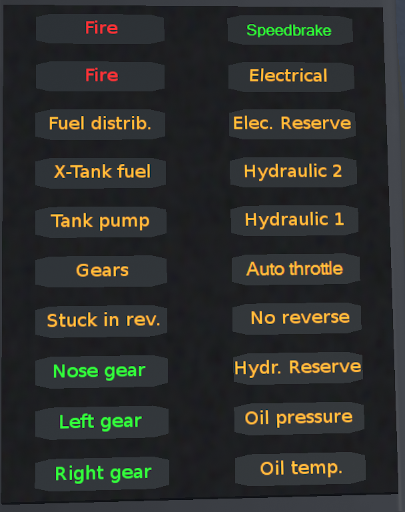
\includegraphics[width=0.45\textwidth]{images/panels/left-warning-panel.png}
  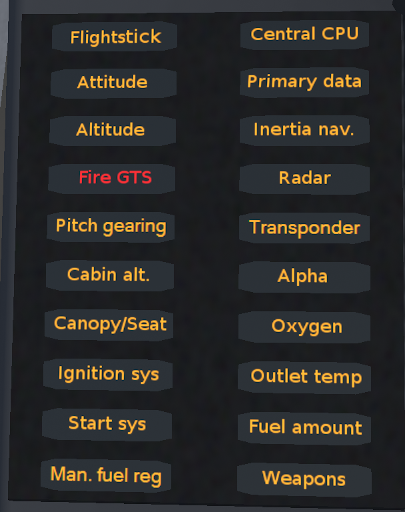
\includegraphics[width=0.45\textwidth]{images/panels/right-warning-panel.png}
  \caption{Left and right warning panels (\cockpitref{fig:front-panel}{item:left-warning,item:right-warning})}
  \label{fig:warning-panels}
\end{figure}

\begin{description}
  \item[Fire (x2)] Engine fire (blinking).
  \item[Fuel distrib] Fuel distribution system failure (blinking, steady if hydraulics failure).
  \item[X-Tank fuel] Blinking: external fuel tank pump failure.
    Steady: external fuel tank pump inactive due to low engine RPM.
  \item[Tank pump] Fuel pump failure (blinking, steady if electrical failure).
  \item[Gear] Blinking: gear up at low speed and altitude.
    Steady: landing gear extending/retracting.
  \item[Stuck in rev.] Thrust reverser engaged and failed (blinking).
  \item[Nose/Left/Right gear] Gear down and locked (steady).
  \item[Speedbrake] Blinking: speedbrakes failure. Steady: speedbrakes extended.
  \item[Electrical] Failure in electrical system (blinking).
  \item[Elec. Reserve] Emergency ram air turbine failure, or abnormal engagement (blinking).
  \item[Hydraulic 1/2] Low pressure in hydraulic systems (blinking).
  \item[Auto throttle] Steady: normal auto-throttle disengagement.
    Blinking: abnormal auto-throttle disengagement, or failure.
    Pull auto-throttle to off (up) position to reset.
  \item[No reverse] Failure of thrust reverse of tertiary air intake (blinking).
  \item[Hydr. Reserve] Low pressure in backup hydraulic system (blinking).
  \item[Oil pressure] Low pressure in engine oil system (blinking).
  \item[Oil temp.] High engine oil temperature (blinking).
  \item[Flightstick,Attitude,Altitude] Abnormal disengagement of corresponding or higher autopilot mode (blinking).
    To reset, acknowledge master warning, then press any autopilot button.
  \item[Fire GTS] Fire in engine start system (blinking).
  \item[Pitch gearing] Failure in elevator reduction gearing (blinking).
  \item[Cabin alt.] Low cabin pressure (blinking).
  \item[Canopy/Seat] Failure of canopy or ejection seat (blinking).
  \item[Ignition sys] Engine ignition active (blinking).
  \item[Start sys] Engine start sequence in progress (steady).
  \item[Man. fuel reg] Automatic fuel regulation disengaged (steady).
  \item[Central CPU] Main computer failure (blinking).
  \item[Primary data] Flight data computer failure (blinking).
  \item[Inertia nav.] Inertia navigation central aligning (steady).
  \item[Radar] Radar failure (blinking).
  \item[Transponder] Identification transponder failure (steady).
  \item[Alpha] Failure in angle of attack sensor (blinking).
  \item[Oxygen] Oxygen supply closed, or low pressure (blinking).
  \item[Outlet temp] High exhaust gas temperature (blinking).
  \item[Fuel amount] Low fuel quantity (blinking).
  \item[Weapons] Weapon systems failure (blinking).
\end{description}

\section{Other Indicator Lights}
\paragraph{Master Warning (\cockpitref{fig:front-panel}{item:master-warning})}
The master warning consists of two flashing red lights, together with a sound warning.
It generally lights up together with a light on the warning panels.
Pressing the button between the lights acknowledges the warning.
Depending on the nature of the warning,
the master warning lights may remain steady after acknowledgement.

\paragraph{Reverser (\cockpitref{fig:front-panel}{item:rev-light})}
Green light, indicates that the reverser handle
(\cockpitref{fig:front-panel}{item:rev-handle}) is pulled,
and the reverser is armed (but not necessarily active).

\paragraph{Autopilot (\cockpitref{fig:front-panel}{item:autopilot})}
Three green pushbuttons/lights.
Used to select one of the autopilot modes: stability assist (STICK/SPAK),
attitude hold (ATT), altitude hold (ALT/HÖJD).
When an autopilot mode is active, the light for it and any lower mode are lit.
The lights can blink to indicate special flight conditions under which the
autopilot is not fully functional.

\paragraph{Autothrottle (\cockpitref{fig:front-panel}{item:autothrottle-lights})}
The orange A/T (AFK) light indicates that autothrottle is active.
The pushbutton/light 15,5\textdegree{} is used to select the high-alpha landing mode
(requires landing gear down).

\paragraph{Transonic / Low Speed Reverse(\cockpitref{fig:front-panel}{item:transonic})}
Yellow light, indicates that the aircraft is in the transonic regime.

On the ground, it instead lights up when the reverser is active at low airspeed,
indicating a risk of hot air ingestion and engine fire.
A low throttle setting (EPR<1.4) should be maintained in this case.

% Not implemented
%\paragraph{Weapon Released (\cockpitref{fig:front-panel}{item:release})}
%\paragraph{Fast Reset (\cockpitref{fig:front-panel}{item:fast-reset})}}


\AJSonly{
\chapter{Control Panels}
\section{Main Mode Selector}
The main mode selector knob \cockpitref{fig:left-panel}{item:main-mode}
is located on the radar panel, next to the throttle.
It selects an aircraft main operation mode, corresponding to different phases of a flight.
The knob can be rotated with the keybindings \keys{M} / \keys{\shift+M}.

\subsection{Main Modes}
\begin{description}
  \item[FK/TST] Built-in test. Not implemented (does the same as BER/PRE).
  \item[BER/PRE] Standby mode. Used during start-up and taxi.
    The displays (HUD and CI) are turned off in this mode.
  \item[NAV] Navigation mode. Used during most of the flight, including takeoff.
  \item[ANF/CBT] Combat mode. Allows using weapons. See \cref{chap:weapons}.
  \item[SPA/REC] Reconnaissance mode. Not implemented (does the same as NAV, minus the takeoff submode).
  \item[LANDING NAV] Instruments landing mode. Requires the destination airport to be set in the route manager.
    It enables inertia navigation guidance for the approach, and ILS guidance for the final.
  \item[LANDING P/O] Visual landing mode.
\end{description}

\subsection{Example of Use}
A typical flight may use the following modes.
Initially, the mode is BER/PRE.
Shortly before takeoff (e.g.\ when entering the runway), the mode is switched to NAV.
In order to use weapons, the mode is switched to ANF/CBT,
then back to NAV when resuming normal flight.

In general, LANDING mode is selected up to 20km away from the destination.
LANDING NAV mode will give indications to follow a full approach pattern,
and enables ILS guidance for final, if available.
LANDING P/O simply gives a target glide slope indicator on the HUD, to help with visual landing.
One can also begin the approach in LANDING NAV mode,
and later switch to LANDING P/O to finish the approach visually.

\subsection{Alternative Landing Approaches}
For the LANDING NAV mode, the approach pattern can be changed 
by the following operations (called `flip-flop').
\begin{itemize}
  \item Switching to LANDING P/O, then back to LANDING NAV select the short approach mode,
    with a 10km final instead of a 20km final.
  \item Switching to NAV, then back to LANDING NAV resets the landing mode.
    A new approach pattern starts, with a long (20km) final.
    (any non-landing mode can be used instead of NAV).
\end{itemize}
}


%\chapter{Displays}

%\chapter{Systems}

% TODO: https://github.com/NikolaiVChr/flightgear-saab-ja-37-viggen/issues/120
%\section{Course Correction for Magnetic Deviation}
%Like in the real Viggen there are two ways to set the course correction, which makes sure that the instruments show true North instead of magnetic North (e.g. in north Norway the deviation is larger than 12\degree):
%\begin{itemize}
% \item Automatic: Simplified the computer averages the deviation between measured between 110 and 200 km/h during take-off.
% \item Manual: Make sure your airplane is properly aligned with the runway. Press FIXME. The reason for doing it manually is if the runway is slippery or there are strong crosswinds, which might change the way the nose points and therefore give a wrong deviation measurement. 
%\end{itemize}

%Please note that the computer in the real Viggen also makes some comparisons with the stored runway heading(s) to decrease the risk of failures. Warning light \emph{NAV SYST} would lit up. However, this is not modelled in FlightGear. 

%\AJSonly{Reference: [AJS\_1, sec. 20, ch. 3.4, p. 312]}

\part{Operation}
\chapter{Generic FlightGear Operations}
\section{Key Bindings}
A summary of the key bindings can also be found in \menu{Help>Aircraft Help}.

\paragraph{General}
\begin{description}
\AJSonly{
  \item[\keys{M} / \keys{\shift+M}] Rotate main mode selector knob clockwise/counterclockwise.
  \item[\keys{K} / \keys{J}] Extend/retract airbrakes (press for ca.\ 2s for full extension).
    When the landing gear is down, airbrakes retract as soon as \keys{K} is released.
  \item[\keys{\ctrl+B}] Toggle airbrakes (simplified airbrakes control).
    When the landing gear is down, airbrakes retract as soon as \keys{\ctrl+B} is released.
}
  \item[\keys{\backspace}] Toggle thrust reverser
  \item[\keys{\shift+R}] Set reference altitude (goal altitude displayed on HUD).
  \item[\keys{\shift+H}] Cycle HUD brightness.
  \item[\keys{I}] Display target type/callsign on \ifbool{AJS}{HUD}{MI}.
  \item[\keys{\shift+I}] Toggle between english/imperial and swedish/metrics display modes.
  \item[\keys{\shift+PageUp} / \keys{\shift+PageDown}] Raise/lower seat position.
  \item[\keys{O}] Open/close canopy.
  \item[\keys{\ctrl+E} $\times3$] Eject
  \item[\keys{J}] Jettison drop tank (in flight only).
  \item[\keys{\shift+S}] Acrobatic smoke.
\JAonly{
  \item[\keys{\shift+Y}] Engage landing mode.
}
  \item[\keys{\ctrl+Y}] Ask tower for landing airport information (requires runway selected in route manager).
\end{description}

\paragraph{View}
\begin{description}
  \item[\keys{Q}] Reset view.
  \item[\keys{\ctrl+Q}] Zoom on radar display.
  \item[\keys{\ctrl+\shift+Q}] Zoom on HUD.
\end{description}

\paragraph{Autopilot}
\begin{description}
  \item[\keys{\ctrl+T}] Autopilot stability assist mode.
  \item[\keys{\ctrl+W}] Autopilot attitude hold mode.
  \item[\keys{\ctrl+A}] Autopilot altitude hold mode.
  \item[\keys{\ctrl+D}] Disengage all autopilot modes.
  \item[\keys{\ctrl+S}] Toggle autothrottle lever.
  \item[\keys{\ctrl+G}] Autothrottle quick disengage.
  \item[\keys{\ctrl+\arrowkeyleft} / \keys{\ctrl+\arrowkeyright}] Trim yaw, or adjust autopilot heading/bank angle.
\end{description}

\paragraph{Radar Controls}
\begin{description}
  \item[\keys{R}] Toggle radar.
  \item[\keys{Y}] Use flight controls to controls radar cursor (cf.\ \cref{sec:cursor})
  \item[\keys{[} / \keys{]}] Decrease/increase radar range (positions: 15km, 30km, 60km, 120km).
  \item[\keys{N}] Select next radar track.
  \item[\keys{\shift+N}] Select center-most radar track.
  \item[\keys{\ctrl+N}] Set next waypoint as radar target.
  \item[\keys{\shift+F}] Unlock radar track.
\end{description}

\paragraph{Combat}
\begin{description}
\JAonly{
  \item[\keys{H}] Toggle master arm.
}
  \item[\keys{C}] Cycle weapons.
  \item[\keys{U}] \ifbool{AJS}{Select IR missile}{Select cannon}
\AJSonly{
  \item[\keys{\shift+U}] Uncage IR missile seeker (requires lock).
    Held: cage/reset IR missile seeker.
}
  \item[\keys{\shift+E}] Toggle trigger safety.
  \item[\keys{E}] Fire weapon.
  \item[\keys{Q}] Release flare/chaff.
\end{description}

\subsection{Radar Stick Controls}
\label{sec:cursor}
The radar stick is used to control the cursor on the \ifbool{AJS}{CI}{MI and TI}.
There are three ways to control it:
\begin{itemize}
  \item Enable the option \menu{\ifbool{AJS}{AJS-37}{JA-37Di}>Options>Arrow keys control radar cursor}
    and use the arrow keys.
  \item Add joystick bindings to control the cursor.
    This can be done under \menu{File>Joystick Configuration},
    the controls are named \menu{Cursor Horizontal}, \menu{Cursor Vertical}, and \menu{Cursor Click}.
    Alternatively, manually edit joystick configuration files to bind the properties
    \begin{alltt}
/controls/displays/cursor-slew-x
/controls/displays/cursor-slew-y
/controls/display/cursor-click
    \end{alltt}
  \item Press \keys{Y} to use the main flight controls
    (joystick, mouse, arrow keys, whatever you use to control the aircraft)
    to instead control the cursor.
    In this mode, elevator and aileron controls are used to move the cursor,
    and the trigger \keys{E} is used to click.
    Normal flight controls are restored by pressing \keys{Y} again.
    A ground collision warning will also immediately restore normal flight controls.

    Consider using autopilot when controlling the cursor in this way.
\end{itemize}

\AJSonly{The same controls are also used for the Rb 05A remote controlled missile.}

\section{\variant{} Menu}
The menu \menu{\ifbool{AJS}{AJS-37}{JA-37Di}} contains Viggen-specific dialogs and menus.
The following entries are present.
\begin{description}
  \item[\menu{Select Livery}] There is a variety of liveries available, both historical and fictional.
  \item[\menu{Auto start/stop}] Lets you start and stop the plane without needing to switch switches etc.\ yourself.
    The progress is shown in the top centre of the screen in blue text.
    The final notification of the start-up sequence is `Engine ready'.
    The shut-down sequence is done, when the aircraft is dark.
  \item[\menu{Repair}] Repairs system failures when on the ground.
    In case of a full crash, this option is mostly useless;
    one should restart instead, for instance with \menu{Location>Select Airport}.
  \item[\menu{Fuel/Loadout}] The fuel slider allows quick selection of fuel quantity,
    while ensuring proper fuel balance.
    Fuel quantity is indicated as a percentage, which corresponds to the fuel gauge reading.
    A level of 100\% corresponds slightly less than full internal tanks.

    The loadout selection buttons in the rest of the screen allow
    fast selection of preset historical weapon loadouts.
    The button \menu{Clean loadout} removes any loaded weapon.
    The button \menu{Reload ammo/flares} reloads ammunition
    for guns, rocket pods and bomb racks, as well as flares.

    Compared to the standard dialog \menu{Equipment>Fuel and Payload},
    this dialog is quicker and ensures some realism, but allows less choices.
  \item[\menu{Performance monitor}] Display aircraft performance (mostly for development).
  \item[\menu{Systems monitor}] Display internal status of some systems (mostly for development).
  %\JAonly{\item[\menu{Friends and Foes}] TODO
  %}
  \item[\menu{Toggle external power}] External electrical power, normally used for startup.
    An electrical power truck is shown to the right of the aircraft when enabled.
    Only available when fully stopped.
  \item[\menu{Options}] Viggen specific configuration options, see \cref{sec:options-dialog}.
\end{description}

\section{\variant{} Options}
\label{sec:options-dialog}
The dialog \menu{\ifbool{AJS}{AJS-37}{JA-37Di}>Options} contains the following configuration options.
\begin{description}
  \item[\menu{HUD line width}] Allows to improve HUD visibility if necessary.
  \item[\menu{G-suit quality}] Changes resistance to blackout under high G-load.
  \item[\menu{Cockpit labels in Swedish}] Enable historical Swedish cockpit,
    instead of the English translation.

    The cockpit translation is far from complete: parts of the cockpit will be
    in English, and others in Swedish, regardless of this setting.

    This option is for \emph{physical labels} only,
    and should not be confused with the next one which affects displays.
  \item[\menu{HUD/TI in metric units and Swedish}]
    Change the unit system and language used in displays.  Shortcut: \keys{\shift+I}.

    This option is for \emph{displays} only
    and should not be confused with the previous one which affects physical displays.
\JAonly{
  \item[\menu{TI Display: show non-functional menu items}]
    On the TI display (Horizontal Situation Display),
    show menus non-implemented menus.
  \item[\menu{TI Display: use Internet to fetch map}]
    Enable download of the world map displayed on the TI (Horizontal Situation Display).
}
  \item[\menu{Rust on fuselage}]
    Purely visual. Only available when using the Atmospheric Light Scattering (ALS) FlightGear renderer.
  \item[\menu{Rust in cockpit}]
    Purely visual. Only available when using the Atmospheric Light Scattering (ALS) FlightGear renderer.
  \item[\menu{Arrow keys control radar cursor}]
    When enabled, the arrow keys will control the radar stick to move the cursor on the different displays.
    When disabled, the arrow keys are used for flight controls (FlightGear default behaviour).
    Cf.\ \cref{sec:cursor} for more details regarding cursor controls.
  \item[\menu{Enable multiplayer damage}]
    Allows to deal and receive damage from other compatible aircrafts
    (other Viggens, F-14, F-15, F-16, M-2000, MiG-21, etc.) in multiplayer.
    This requires \emph{both} involved aircraft to enable damage.

    For fairness, this option can only be toggled when stopped on the ground.
    It also enforces some realism options: blackout, normal simulation speed,
    no external views, and disabling fuel, payload and repair menus while in flight.
\end{description}


\chapter{Standard Procedures}
To come! Please check FlightGear built-in checklists
\menu{Help>Aircraft Checklists} in the meantime.

%\chapter{Emergency Procedures}

\chapter{Weapons Operation}
\label{chap:weapons}
\section{Generalities}
The generic weapon employment procedure is the following.
\begin{enumerate}
  \ifbool{AJS}{
  \item Main mode selector to ANF/CBT.
    (\cockpitref{fig:left-panel}{item:main-mode}, shortcuts \keys{M}/\keys{\shift+M}).
  }{
  \item Master arm on (shortcut \keys{H}).
  }
    Combat mode will only be enabled in the air with gear up and locked.
    In combat mode, the HUD presentation changes slightly.
    Weapon type is indicated in the lower left, ammunition in the lower right.
  \item Select the weapon type with \keys{C}, or \keys{U} to select
    \ifbool{AJS}{IR missiles}{the cannon}.
  \item Unsafe the trigger with \keys{\shift+E}.
    This arms the selected weapon.

    For gun, rockets, and bombs, the aim (or CCIP) indicator appears on the HUD.
    Missiles will start looking for a target.

    Trigger unsafing is normally done once the target is in sight or on radar,
    and the choice to engage it has been made.
  \item For missiles, ensure that the missile has locked onto the target.
  \item Fire the weapon with \keys{E}.
  \item Secure the trigger with \keys{\shift+E}.
\end{enumerate}

\subsection{Trigger Safety Usage}
The trigger safety role is not merely to prevent unintentional fire.
It is an import part of the fire control system:
as a general rule, the trigger safety arms the selected weapon.
As a consequence, improper use of trigger safety will prevent weapon usage.
Below are some errors and caveats to look out for.
\begin{itemize}
  \item Unsafing the trigger arms the selected weapon.
    Thus it must be done \emph{after} entering combat mode and selecting the desired weapon.
  \item If a new weapon is selected while the trigger is unsafe,
    the new weapon will not be armed (until the trigger is safed and unsafed again).

    Similarly, if the trigger is kept unsafe while exiting combat mode,
    upon re-entering combat mode, the weapon will not be armed.
  \item After firing a missile, the next missile is only selected upon securing the trigger.
    It is not possible to fire several missiles in succession without securing the trigger in-between.
\end{itemize}

\AJSonly{
\section{Rb 05A}
The Rb 05A is a remote-controlled missile.
It is primarily intended for use against ground and naval targets,
but can also be used against slow-manoeuvring air targets thanks to a proximity fuse.
The missile is guided visually by the pilot.
A flare at the back of the missile helps the pilot to keep sight of it (\cref{fig:rb05-flare}).

\begin{figure}
  \centering
  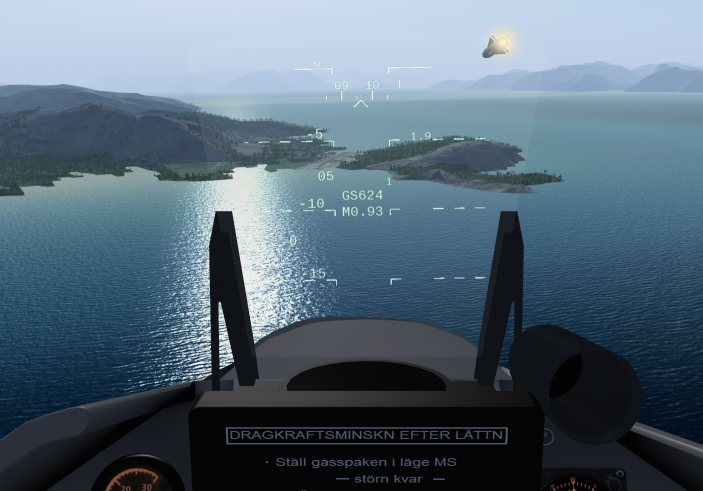
\includegraphics[height=0.3\textwidth]{images/weapons/rb_05a_start_popup.png}
  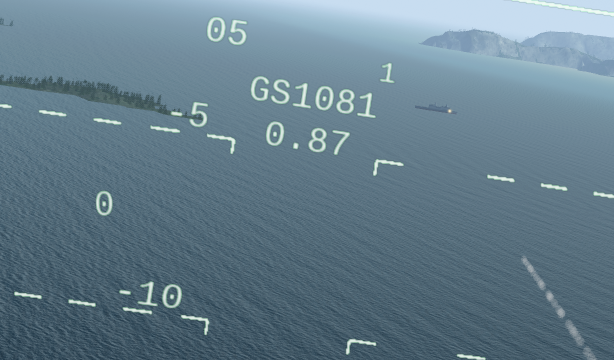
\includegraphics[height=0.3\textwidth]{images/weapons/rb_05a_before_impact_ship.png}
  \caption[Rb 05A flare for visual guidance]{Rb 05A flare for visual guidance.
    On the left, the missile is entering the pilot's field of view just after launch.
    On the right, the missile is about to hit the target ship,
    and the missile flare is visible over the ship
  }
  \label{fig:rb05-flare}
\end{figure}

In FlightGear, the Rb 05A uses the same controls as the radar stick, cf.\ \cref{sec:cursor}.\footnote{%
  In the real Viggen, a separate control stick on the right console was used.
}

\subsection{Procedure}
\begin{enumerate}
  \item Main mode selector to ANF/CBT.
    (\cockpitref{fig:left-panel}{item:main-mode}, shortcuts \keys{M}/\keys{\shift+M}).
  \item Select the Rb 05A (cycle weapons with \keys{C}).
  \item Once in firing position, consider engaging autopilot in ATT or HÖJD/ALT mode to reduce pilot workload.
  \item Identify the target visually.
  \item Unsafe the trigger and fire within 9km of the target.
  \item After 1.7s, missile controls are enabled
    (cf.\ \cref{sec:cursor} for control methods).
    At this point, it should be well within the pilot field of view.
  \item When the missile hits, take evasive manoeuvres, secure the trigger, and switch to NAV mode.
\end{enumerate}

Remarks.
\begin{itemize}
  \item Recommended speed is 700-1150 km/h.
  \item Recommended attitude is a level flight or slight dive,
    so as to not loose sight of the target and the missile.
  \item Recommended altitude is 300-400 meters above ground.
  \item The target do not need to be directly in front of the aircraft
    as the missile can be guided considerably to the side.
    However, doing so makes it harder to aim the missile, and reduces effective range.
  \item The missile flies for ca.\ 24 seconds, giving it a maximum effective range of ca.\ 9 km.
  \item It is easiest to aim the missile using the collimation principle:
    try to keep the missile flare covering the target at all time.
\end{itemize}
}
\end{document}

%\url{https://www.aef.se/Flygvapnet/Tidskrifter/FV_Nytt/Flygvapennytt_1993-2.pdf} has an article and 2 pictures about the automatic aiming mode for the cannon in the JA version (in Swedish).

\appendix

\chapter{References}

A comprehensive book in English covering all variants is \glqq Saab 37 Viggen --- The ultimate portfolio\grqq by Jan Jørgensen (published in 2014 by \href{http://www.nordicairpower.com/}{Nordic Airpower}).

\subsection{Original Manuals}
A significant part of the original manuals are available on the internet, and in recent years also many of the formerly classified chapters (as far as the information is not still valid due to (re-)use in the Gripen) have been become available. As the Viggen could not be sold to other countries\footnote{Austrian pilots went through a training programme on the Viggen to familiarise with modern combat airplane, but never bought it}, a significant part of the text and illustrations are in Swedish.

The following manuals are core to the understanding of flying a Viggen in military operations. Where possible, references are made in this manual to text elements in the original manuals(e.g. [AJS\_Del1, sec. 20, ch. 3.4.2, p. 312]). Also, this manual does typically not repeat illustrations from the original handbooks, but shows a screenshot from the simulation instead, so you can compare.

\begin{table}[!th]
\begin{tabular}{|l|l|c|r|}
\hline
Ref & Title & Date & Pages \\
\hline
AJ\_Del2 & FPL AJ37 Speciell Förarinstruktion Del 2 kap 1 (M5800--370011) & 1975--02--01 & 181 \\
AJS\_Del1 & FPL AJS37 Speciell Förarinstruktion Del 1 (M5800--370011) & 1994--11--15 & 517 \\
AJS\_Del2 & FPL AJS37 Speciell Förarinstruktion Del 2 (M5800--370011) & 1994--11--01 & 222 \\
AJS\_Del3 & FPL AJS37 Speciell Förarinstruktion Del 3 (M5800--370011) & 1994--11--15 & 295 \\
JA\_Vol1 & Flight Manual A/C JA37 Volume 1 (M5800-370051) & 1999--01--20 & 497 \\
\hline
\end{tabular}
\caption{Overview of flight manuals from the original Viggen}
\end{table}

\subsection{FlightGear Related}
\begin{itemize}
\item The \href{http://wiki.flightgear.org/Saab_37_Viggen}{FG wiki article} contains a comprehensive feature overview, links to forum articles etc. However, the wiki is not always up to date.
\item \href{http://opredflag.com/}{Operation Red Flag (OPRF)} is a FlightGear military simulation community discussing, developing and using many of the combat features in the Viggen.
\item On Discord there is a dedicated \href{https://discord.gg/jc5pSM5}{Viggen server} and a \href{https://discord.gg/SmGFnJN}{OPRF server}. Say hello and discuss the Viggen's features, development and your flight experience. Preliminary help with issues can be gotten as well, confirmed issues should be reported in the Viggen's \href{https://github.com/NikolaiVChr/flightgear-saab-ja-37-viggen/issues}{issue tracker} for resolution.
\item The \href{https://www.youtube.com/playlist?list=PLogi97V-ki0GfCLqimTtIq9RIVcm-GRFE}{Flightgear Saab 37 Viggen YouTube Playlist} includes amongst others a set of tutorial videos featuring the JA and the AJS variant.
\end{itemize}

\subsection{Other Combat Flight Simulators}
Both \href{https://www.digitalcombatsimulator.com/en/index.php}{DCS} and \href{https://www.benchmarksims.org/}{BMS Falcon} have flyable Viggens. Especially for DCS there is an abundance of resources available on the internet (e.g. YouTube). Please note that while there can be valuable additional information and context provided in content from other simulators, the capabilities modelled will differ.

\subsection{Swedish Documentation Sites}
\begin{itemize}
\item Arboga Elektronikhistoriska Förening: \url{https://www.aef.se}, e.g. 
\begin{itemize}
\item \href{https://www.aef.se/Avionik/Notiser/PS-37/PS-37A.htm}{Spanings- och siktesradar PS-37/A (for the AJS)}
\item \href{https://www.aef.se/Avionik/Notiser/Siktesradar_PS-46_1.htm}{Flygradarinstallation JA37 ---Siktesradar PS46} (includes links to 2 articles from Ericsson)
\item \href{https://www.aef.se/Flygvapnet/Tidskrifter/FV_Nytt/FVN_oversikt.htm}{FlygvapenNytt 1960 – 2003}: \url{https://www.aef.se/Flygvapnet/Tidskrifter/FV_Nytt/Flygvapennytt_1991-2.pdf} announced the AJS Viggen and \url{https://www.aef.se/Flygvapnet/Tidskrifter/FV_Nytt/Flygvapennytt_1994-4.pdf} had follow-up articles.
\end{itemize}
\item Digitalt Museum: \url{https://digitaltmuseum.se/}:
\begin{itemize}
\item Aeroseum Göteborg: \url{https://digitaltmuseum.se/owners/S-AER}
\item Flygvapenmuseum: \url{https://digitaltmuseum.se/owners/S-FV}
\item Teknikland: \url{https://digitaltmuseum.se/owners/S-TL}
\item Sveriges militärhistoriska arv: \url{https://digitaltmuseum.se/owners/S-MHA}
\end{itemize}
\end{itemize} 


\begin{landscape}
\chapter{Viggen Related Videos}
The following selection of videos has been made based on operational content or visibility of details. There exist many more videos --- some of which with higher quality from recent air shows. If you miss a video below, let us know.

\begin{table}[!th]
\begin{tabular}{|p{5cm}|c|c|c|p{9cm}|}
\hline
Title & Length & Subtitles & Year & Comments \\
\hline

\href{https://www.youtube.com/watch?v=kBq5qA8r4dA}{SF/SH37 \& JA37 VIGGEN at F13 Wing} & 18 min & yes & 2000 & Mostly about the reconnaissance and photo version\\
\href{https://www.youtube.com/watch?v=0sRACNVVmpE}{Saab 37 Viggen 2001 1-2} & 15 min & no & ?? & Historic part plus early versions\\
\href{https://www.youtube.com/watch?v=pAPteuBsRGg}{Saab 37 Viggen 2001 1-2} & 14 min & no & ?? & Mostly about the evolution of the JA. Some footage of HUD and CI/TI screens.\\
\href{https://www.youtube.com/watch?v=fmqXa0oetUA}{VI FLÖG HÅRT OCH STRIDSMÄSSIGT} & 15 min & no & ?? & A fighter pilot tells stories\\
\href{https://www.youtube.com/watch?v=ErK3zaNRccE&}{Jaktviggenpilot på Bråvallajakten} & 14 min & no & 1989 & A day in the live of a fighter pilot\\
\href{https://www.youtube.com/watch?v=qaNt9_sQdGI}{Kurvstrid (Dogfight) SAAB JA37C VIGGEN} & 8 min & yes & ?? & Various dogfights with some HUD visibility\\
\href{https://www.youtube.com/watch?v=oB6-jJEWjWk}{S som i Speed - Göran flyger Viggen} & 6 min & no & 1996 & Some low level flying\\
\href{https://www.youtube.com/watch?v=gwgJNdWZlj0}{SH-37 Viggen Sea Surveillance} & 4 min & n/a & ?? & Some nice sequences of the AJS CI and a few glipse of the HUD\\
\href{https://www.youtube.com/watch?v=mgPS5-SbI0c}{Viggen attackuppdrag} & 2 min & no & ?? & Attack with rockets using pop-up method. Some sequences of the HUD.\\
\href{https://www.youtube.com/watch?v=eQjAp7bTnUg}{Kalla Krigets Fordon avsnitt 6: SAAB 37 Viggen} & 9 min & no & 2016 & A bit of history and relation between the plane and the road base system. During the very last seconds some close-up sequences of the CI.\\
\href{https://www.youtube.com/watch?v=slm9ksxU0HY}{Viggen Road base exercise} & 6 min & n/a & ?? & As the title says.\\
\href{https://www.youtube.com/watch?v=hWrsP3hq5M8}{AJ-37 Viggen Low Level Flying} & 4 min & n/a & ?? & As the title says. Some HUD sequences incl. rocket attack.\\
\href{https://www.youtube.com/watch?v=UOszNlNeRVs}{SAAB 37 Viggen} & 4 min & n/a & ?? & Some nice air ballet plus a few sequences of the CI.\\
\href{https://www.youtube.com/watch?v=IbsYsUvCy7s}{Rörlig klargöring JA37 Arlanda} & 43 min & no & 1996 & Ground operations of JA 37 on an improvised stand at Arlanda airport\\
\href{https://vimeo.com/60091080}{Viggen i Älskar, älskar inte} & 4 min & no & ?? & Excerpts from the feature film, Älskar, älskar inte. Nice dogfighting between JA and AJS plus some CI sequences\\
\href{https://www.youtube.com/watch?v=eT00_OVrv7o}{JA-37 and SK-37E Night Ops} & 7 min & no & ?? & Night flying with good pictures of exhaust, navigation and beacon lights\\
\href{https://www.youtube.com/watch?v=0ocSUd9_5Tw}{JA37 F21 1982-2004} & 17 min & no & ?? & Around min 5 and 15 there are longer sequences of the HUD in weapons mode (JA variant)\\

\hline
\end{tabular}
\caption{Selected videos featuring the Viggen. Unless described otherwise in the comments, the language is Swedish}
\end{table}

% Videos watched but not found interesting enough
% \href{https://www.youtube.com/watch?v=rFZKvO95bQ0}{2018-10-17 Svensk stridspilot under det kalla kriget}
% \href{https://www.youtube.com/watch?v=RHVzkVwI68w}{Vetenskapens Värld - Viggen} Mostly project and politics history until first viggen operational
% \href{https://www.youtube.com/watch?v=M8HF1gH0MPc}{37 Viggen - The Power of Viggen!} Mostly flight display
% \href{https://www.youtube.com/watch?v=Z_EnkvE6LZA}{Fredens Hav}
\end{landscape}

